\documentclass[jou,apacite]{IEEEtran}
\usepackage{amsfonts}
\usepackage{amsthm}
\usepackage{tabu}
\usepackage{amssymb}
\usepackage{mathtools}
\usepackage{relsize}
\usepackage[font=footnotesize]{subfig}
\usepackage{hyperref}
\usepackage{minted}
\setminted{fontsize=\scriptsize, frame=single, breaklines=true}

\usepackage{graphicx}
\graphicspath{ {../images/} }
\setlength\parindent{0pt}

\title{Scala - A Powerful and Scalable Function-Objective Programming Language}

\author{Troy Hu and Benjamin Killeen} % alphabetical by last name

\begin{document}
\maketitle    

\begin{abstract}
Insert abstract here.
\end{abstract}                     

\section{Introduction}
\label{sec:intro}

Software components are simply self-contained parts of software used by larger
parts or entire applications. Modern software typically relies on many common
components like hashable types or iterable data structures to use as building
blocks. Component abstraction enables the generalization of implementation for
these features, greatly reducing duplication of effort. It is one of the most
powerful tools in the programmer's utility belt, a fact which the designers of
the Scala programming language aimed to exploit \cite{odersky2004overview}. In
the early 2000s, existing languages had little support for type-sound component
abstraction, including widely used languages like Java and C\#. Odersky \emph{et
  al.} address this shortcoming with a language that combines elements of
object-oriented and functional programming in a statically typed
environment. Scala, which gets its name from ``scalable,'' provides a powerful
interface for abstraction within a development framework intended for mass
adoption.

In pursuit of usability, Scala borrows many syntactic elements from Java and
C\#, and it integrates smoothly with components from these languages. In fact,
the Scala library includes standard Java objects like \texttt{java.lang.String},
as shown in Lst.~\ref{lst:print}. Scala code can take advantage of existing
implementations in Java, and in the end it compiles to Java bytecode, making
Scala packages available to Java programmers. At the same time, Scala maintains
a distinct programming paradigm from either Java or C\#. It discards some
features from these languages, and it develops completely novel ideas from the
$\nu$Obj calculus \cite{odersky_nominal_2003}. The example in
Lst.~\ref{lst:print} highlights syntactic similarities between Java and Scala,
comparing two implementations of the same program. Note how Java prepends type
declarations before terms, whereas Scala affixes type declarations using the
\texttt{:} operator. This and other changes effect a terser, more expressive
syntax overall.

\begin{listing}
  \centering
  \inputminted{Java}{../examples/PrintExample.java}
  \inputminted{Scala}{../examples/PrintExample.scala}
  \caption{Notice how Scala's general syntax and structure are similar
    to Java's. At the same time, there are some visible differences, e.g., unit
    is returned in the Scala implementation instead of void in the Java
    implementation.}
  \label{lst:print}
\end{listing}

Of course, Scala's foremost strength comes from its typing system. Abstract
class definitions and path-dependent types utilize the $\nu$Obj Calculus,
enabling incredible flexibility through the use of traits and mixins
\cite{odersky_nominal_2003}. Somewhat akin to Java's abstract classes, traits
allow a programmer to rely on abstract methods for common functionalities. For
example, the \texttt{Equiv[T]} trait in Fig.~\ref{lst:equiv} represents an
equivalence relation on the type \texttt{T}, abstracting the definition of
\texttt{eq} on which a concrete method, \texttt{neq} depends. Mixins enable a
class to inherit from multiple traits. For instance, one might use
\texttt{Equiv} in conjunction with an \texttt{Ordering} trait to represent
separate relations on the same type in one object.

Finally, the uniform object model in Scala provides a cohesive programming
environment. Every Scala value is an object, and every operation is a call to a
method. The boolean \texttt{true}, for example, is a singleton object that
extends (inherits from) the Boolean trait (see
Sec.~\ref{sec:singleton-objects}). At the same time, Scala fits into a
functional programming paradigm. Functions themselves are values, and the syntax
allows for SML-like decomposition and pattern matching. These features result in
a powerful language with a unified programming experience.

% 3. related work
\section{Related Work}
\label{sec:related-work}

\begin{figure*}[h]
  \centering
  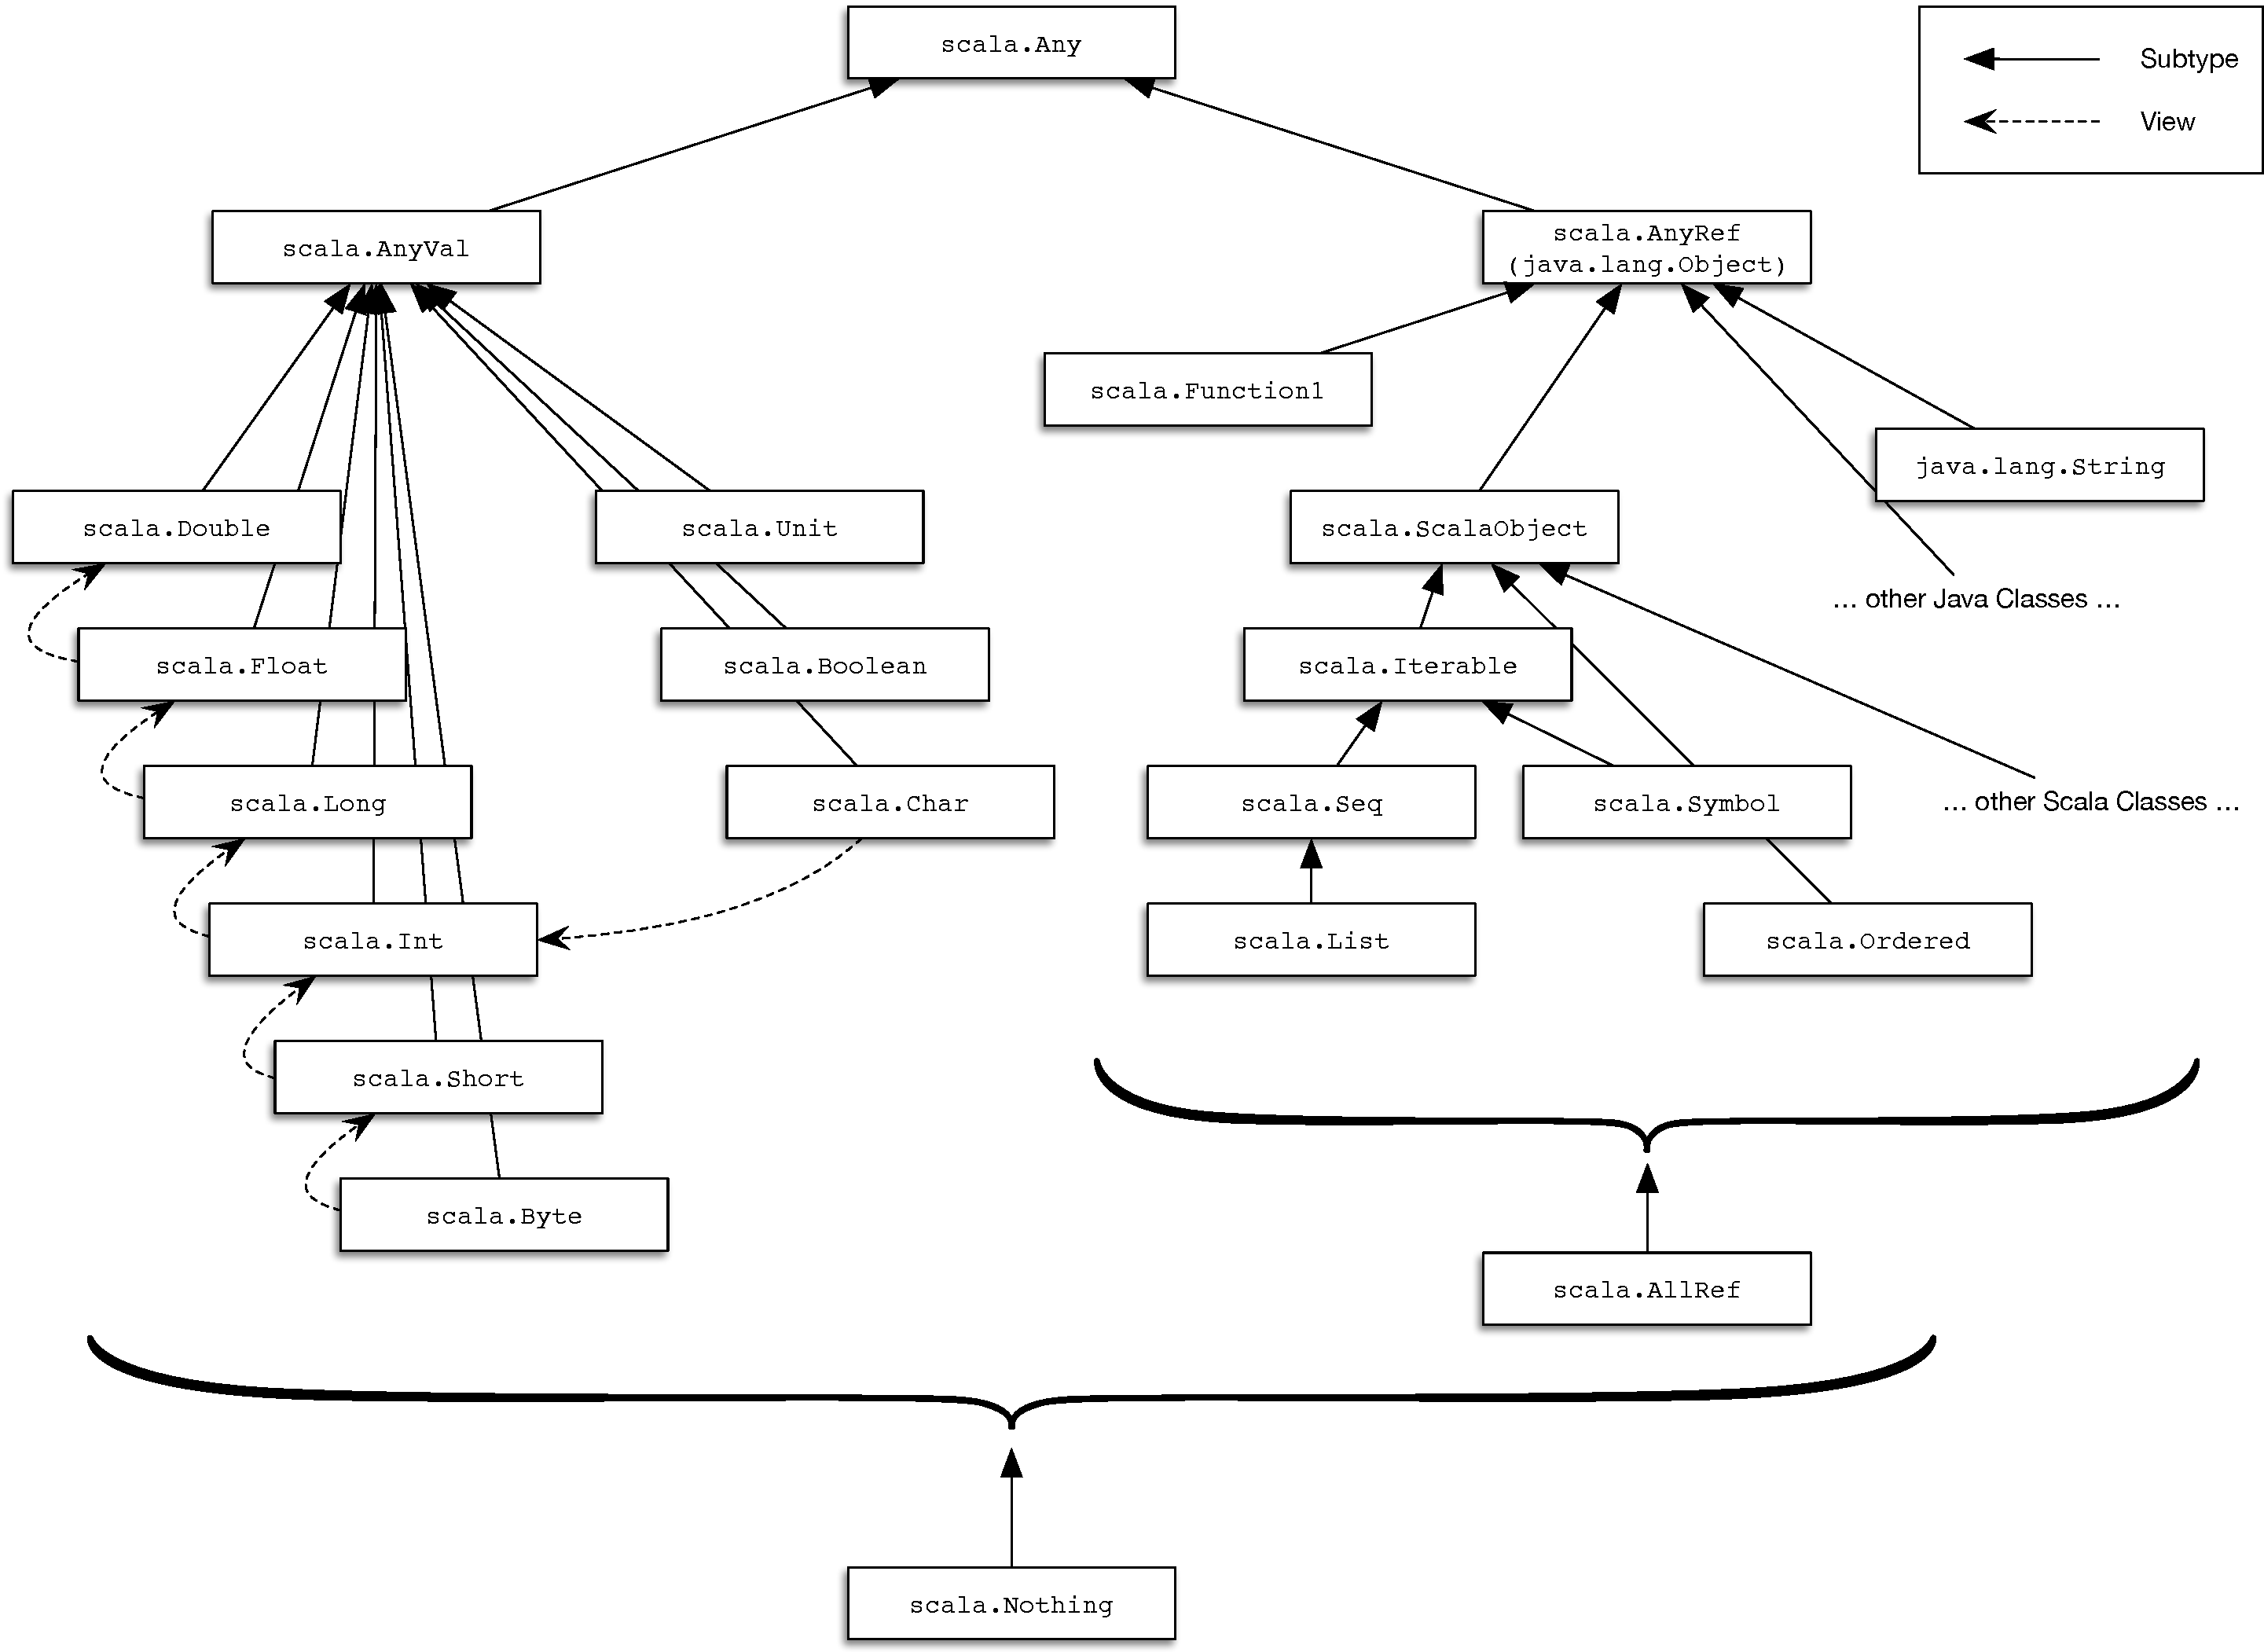
\includegraphics[width=0.9\linewidth]{scala_classes}
  \caption{A visual representation of Scala's class hierarchy}
  \label{fig:example}
\end{figure*} 

The ideas underlying Scala come from a variety of work. First and foremost, the
designers rely on the $\nu$Obj calculus outlined in Odersky \emph{et al.}
(2003) for a theoretical grounding on which they build Scala's robust type
system \cite{odersky_nominal_2003}. Although a thorough discussion of the
$\nu$Obj calculus is beyond the scope of this paper, which focuses on the Scala
language proper, we describe its main points in brief. Additionally, the ideas
in Scala have been replicated or expanded on in more recent work, which we
discuss here.

The $\nu$Obj calculus is, broadly, a calculus and dependent type system that
includes classes and objects with types as members
\cite{odersky_nominal_2003}. \emph{Dependent types} rely on some value for
definition, and with this formalism, the $\nu$Obj calculus expresses Java's
inner class system, virtual types, and family polymorphism. Furthermore, it
models SML-style modules and functors, diverging from standard object-oriented
type systems in three fundamental ways:
\begin{enumerate}
\item Objects \emph{and} classes are considered primitive, as opposed to just
  objects.
\item Type checking and evaluation rely on name references rather than object
  records.                     %TODO: check with Troy.
\item Object types are expressible using possibly nominal type components.
\end{enumerate}
These alterations make possible the rigorous blend of object-oriented and
functional styles evident in Scala, differing markedly from traditional
languages like Java and C\#.

% TODO: talk about more related work, including Rust language, more recent
% extensions of Scala's systems.

The remainder of this paper focuses on the practical considerations of
programming in the Scala language.

\section{Programming in Scala}
\label{sec:programming-scala}

Being a fully developed programming language, Scala implements numerous useful
features that encourage modularity and reusability in software. In this section,
we highlight just a few of these, as well as provide an overview of the general
process through which software construction takes place in Scala.

\subsection{Unified Object Model}
\label{sec:unified-object-model}

In Scala, every value is an object and every class is a subtype of the
\texttt{Any} class. Below the \texttt{Any} class, Scala classes can generally be
divided into two groups: value classes that inherit from the \texttt{AnyVal}
class and reference classes that inherit from the \texttt{AnyRef} class. Note
that the value classes that are not \texttt{AnyVal} do not subtype each
other. This means, for example, that the \texttt{Int} class is not a subtype of
the \texttt{Float} class. Scala prevents such subtyping because the language
forces an invariant that when a value is interpreted in a subclass and a super
class, the values's representation does not change. For example, both
\texttt{Int} and \texttt{Float} maintain a \texttt{MaxValue} member. However,
the \texttt{MaxValue} of \texttt{Float} is different from the \texttt{MaxValue}
of \texttt{Int}. Instead, Scala implements \textbf{views} (discussed below)
which allow from implicit conversions from one type to another. As expected of
an object-oriented language, class \texttt{Null} is a subtype of every reference
type. However, since Scala is part functional, the language also has a
\texttt{Nothing} type, which represents an empty type, is a subtype of every
single type. For example, \texttt{Nil} is defined as
\texttt{List[Nothing]}. Note that \texttt{Nothing} allows for the implementation
of options, another functional concept, in Scala.

Another major aspect of Scala's object model is that every operation is the
invocation of a method. For example, \texttt{x + y} is syntactic sugar for
\text{x.+(y)}; \texttt{x} is the receiver object, \texttt{+} is a method defined
in \texttt{x}, and \texttt{y} is the method's argument. In fact, Scala desugars
every identifier between two expressions as a method call of the first
expression. Unlike constructors in Java, Scala constructors just come from the
class name. There is no need for a separate class constructor inside the class
definition. When a class is instantiated with its constructor, the whole body of
the class is executed.

\subsection{Singleton Objects}
\label{sec:singleton-objects}

Scala is very unique in that it implements Singleton Objects. Singleton Objects
are classes that can only have one instance while a Scala program is
running. Such classes are defined almost exactly the same as normal Scala
classes. The only difference is that the \texttt{class} modifier is replaced by
the \texttt{object} modifier. Some examples of singleton objects include: a
class representation of Zero and the PrintOptions example from above. Note that
Singleton Objects are used extensively when Scala uses a Java class. Every
static member of a Java class is stored in a Singleton Object.

\begin{listing}
  \inputminted{Scala}{../examples/Nat.scala}
  \caption{An example outlining Scala classes.}
  \label{lst:nats-example}
\end{listing}

\subsection{Pattern Matching in an Object-Oriented Setting}
Unlike Java and other object-oriented programming languages, Scala implements
pattern matching. That is, Scala provides the programmer with a natural and
functional-like mechanism for ``creating structured data representations similar
to algebraic data types and a decomposition mechanism based on pattern
matching.''

Since Scala is an object-oriented programming language, it does not have
algebraic data types. Instead, Scala creates structured data representations
through the \texttt{\textbf{case}} modifier. If $\textbf{case}$ precedes the
definition of a class, a factory method with the same arguments as the primary
class constructor is automatically defined. For example, in Figure 4, since the
\texttt{\textbf{Num}} and \texttt{\textbf{Plus}} classes are defined with the
\texttt{\textbf{case}} modifier, we can define an “anonymous” \textbf{Num}
object without using the \textbf{new} keyword. As the reader can see, factory
methods are very similar in structure to the constructors of algebraic data
types. In fact, factory methods serve the same purpose as constructors when
pattern matching.

Scala's pattern matching expressions can decompose the factory method
constructors as patterns. The syntax for pattern matching expressions is
\[                              %TODO: make this actual code, not something weird.
    \texttt{x \textbf{case} \{ \textbf{case} $p_1 => e_1$ \textbf{case} $p_1 => e_1$ ... \}}
\]
This syntax matches the object \texttt{x} against the patterns $p_1, p_2, ...$
in order. Each $p_1$ is of the form $FactoryMethod(x_1, x_2, …, x_n)$, where
$FactoryMethod$ refers to the factory method constructors discussed
previously. When a match $p_i$ is found, then $e_i$ is executed. For example, in
Figure 5, the \texttt{eval} function matches \texttt{term} against
\texttt{Num(x)} and \texttt{Plus(left, right)} (the constructors are from Figure
4).

\begin{figure}[h]
  \centering
  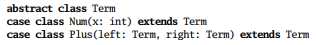
\includegraphics[width=\columnwidth]{abstract_class}
  \caption{example}
  \label{fig:example}
\end{figure}

\begin{figure}[h]
  \centering
  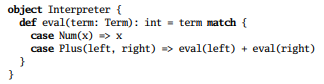
\includegraphics[width=\columnwidth]{pattern_match}
  \caption{}
  \label{fig:example}
\end{figure}

Note: unlike Java, writing a simple language interpreter in Scala is almost as easy as writing an interpreter in SML. Examples of pattern matching being used for an interpreter can be seen in the calculator program we wrote.

\subsection{Views}
Views are used to implictly convert one type to another. A view is implemented
with a method that takes in an arguemnt of one type and returns an object of
another type. The only difference between a view method and a normal method is
that view methods require the \texttt{implicit} modifier, which goes before the
method definition. This modifier allows the Scala compiler to know that it is
the implcit conversion method when converting from one type to another. Scala
implictly applies a view to an expression, $e$ of type $T$, when one of the
following cases occur:
\begin{itemize}
\item The expected type of $e$ is not of type $T$.
\item A member selected from $e$ is not a member of $T$.
\end{itemize}  
For example, in Figure 7, \texttt{listToSet} is the view that converts \texttt{GenList[T]} to \texttt{Set[T]}. The compiler inserts applications of the view onto \texttt{xs}.

\begin{figure}
  \inputminted{Scala}{../examples/Set.scala}
  \caption{An example of views and implcit conversions.}
  \label{lst:nats-example}
\end{figure}
% TODO
% singleton objects - DONE

% unified object model -DONE

% pattern matching in an object oriented setting -DONE

\begin{listing}
  \inputminted[firstline=3]{Scala}{../examples/Equiv.scala}
  \caption{A simple equivalence relation Scala.}
  \label{lst:equiv}
\end{listing}

\begin{listing}
  \inputminted[firstline=3]{Scala}{../examples/Ord.scala}
  \caption{An ordering relation in Scala. It is important to distinguish between
    an ordered type and an ordering on that type, of which there can be
    arbitrarily many. \texttt{Ordering[T]} represents the latter.}
  \label{lst:ordering}
\end{listing}

% Abstraction: -NOT DONE
% - subtypes and polymorphism
% - Traits and classes.
%   - A trait do encapsulate state. They just define methods or variables that you
%     have to have but don't provide instantiated values for those.
%   -Classes require implementations or values for everything.

% Multiple inheritance with mixins. (Small paragraph right after abstractions) -NOT DONE

% Views in Scala implement something close to SML's signatures or Haskell's
% typeclasses. -DONE

% 4. report on peano arithmetic calculator.
\section{Engagement: Peano Arithmetic Calculator}
\label{sec:engag-peano-arithm}

% 5. should encapsulate discussion of current status
\section{Discussion}
\label{sec:discussion}

\subsection{Current Status of Work}
After 15 years, Scala has been regularly updated and is currently at stable
release version 2.12.8. Over this period, the core principles of Scala have
remained the same. Scala has achieved widespread adoption in the industry with
companies such as Twitter and Apple utilizing the language. Moreover, Scala has
both a large academic and non-academic user base. The language is often cited or
used in computer science research. In addition, Scala's user community is
thriving. there exist chatrooms, subreddits, and research conferences devoted
entirely to Scala. Numerous libraries, tutorials, and guides are run and
maintained by the community. The main community page can be found at:
https://www.scala-lang.org/community/. A detailed, updated, and easy to read
documentation can be found at: https://docs.scala-lang.org/. Finally, there are
dedicated installers/installation guides for all operating systems at:
\href{https://www.scala-lang.org/download/}{scala-lang.org/download}.


\bibliographystyle{IEEEtran}
\bibliography{scala_project}

\end{document}

%%% Local Variables:
%%% mode: latex
%%% TeX-master: t
%%% TeX-command-extra-options: "-shell-escape"
%%% End:
